% This is LLNCS.DOC the documentation file of
% the LaTeX2e class from Springer-Verlag
% for Lecture Notes in Computer Science, version 2.4
\documentclass{llncs}
\usepackage{llncsdoc}
\usepackage[T2A]{fontenc} 
\usepackage[utf8]{inputenc}
\usepackage[english,russian]{babel}
\usepackage{graphicx}
\usepackage{indentfirst}
\usepackage{hyperref}

%
\begin{document}
\markboth{\LaTeXe{} Class for Lecture Notes in Computer
Science}{\LaTeXe{} Class for Lecture Notes in Computer Science}
\thispagestyle{empty}
\begin{flushleft}
\LARGE\bfseries Instructions for Authors\\
Coding with \LaTeX\\[2cm]
\end{flushleft}
\rule{\textwidth}{1pt}
\vspace{2pt}
\begin{flushright}
\Huge
\begin{tabular}{@{}l}
\LaTeXe{} Class\\
for Lecture Notes\\
in Computer Science\\[6pt]
{\Large Version 2.4}
\end{tabular}
\end{flushright}
\rule{\textwidth}{1pt}
\vfill
%\begin{flushleft}
%\large\itshape
%\begin{tabular}{@{}l}
%{\Large\upshape\bfseries Springer}\\[8pt]
%Berlin\enspace Heidelberg\enspace New\kern0.1em York\\[5pt]
%Barcelona\enspace Budapest\enspace Hong\kern0.2em Kong\\[5pt]
%London\enspace Milan\enspace Paris\enspace\\[5pt]
%Santa\kern0.2em Clara\enspace Singapore\enspace Tokyo
%\end{tabular}
%\end{flushleft}
\newpage
%
\section*{For further information please contact us:}
%
\begin{flushleft}
\begin{tabular}{l@{\quad}l@{\hspace{3mm}}l@{\qquad}l}
$\bullet$&\multicolumn{3}{@{}l}{\bfseries LNCS Editorial Office}\\[1mm]
&\multicolumn{3}{@{}l}{Springer-Verlag}\\
&\multicolumn{3}{@{}l}{Computer Science Editorial}\\
&\multicolumn{3}{@{}l}{Tiergartenstraße 17}\\
&\multicolumn{3}{@{}l}{69121 Heidelberg}\\
&\multicolumn{3}{@{}l}{Germany}\\[0.5mm]
 & Tel:       & +49-6221-487-8706\\
 & Fax:       & +49-6221-487-8588\\
 & e-mail:    & \tt lncs@springer.com    & for editorial questions\\
 &            & \tt texhelp@springer.de & for \TeX{} problems\\[2mm]
\noalign{\rule{\textwidth}{1pt}}
\noalign{\vskip2mm}
%
%{\tt svserv@vax.ntp.springer.de}\hfil first try the \verb|help|
%command.
%
$\bullet$&\multicolumn{3}{@{}l}{\bfseries We are also reachable through the world wide web:}\\[1mm]
         &\multicolumn{2}{@{}l}{\texttt{http://www.springer.com}}&Springer Global Website\\
         &\multicolumn{2}{@{}l}{\texttt{http://www.springer.com/lncs}}&LNCS home page\\
         &\multicolumn{2}{@{}l}{\texttt{http://www.springerlink.com}}&data repository\\
         &\multicolumn{2}{@{}l}{\texttt{ftp://ftp.springer.de}}&FTP server
\end{tabular}
\end{flushleft}


%
\newpage
\tableofcontents
\newpage
%
\section{Introduction}
%
Операторы динамического SQL формируются не на этапе компиляции, а позже -- на этапе выполнения приложения, как строковые выражения. Почти все современные СУБД предоставляют возможность вызова динамических SQL-предложений, которая формально введена в стандарт SQL в 1992 году ~\cite{ISO}.

Необходимость трансляции~\cite{mart} динамических запросов очень актуальна в задачах реинжиниринга информационных систем (ИС), при миграции приложений баз данных и их переносе на другие СУБД ~\cite{NetDbTransform}. При этом требуется транслировать с одного диалекта SQL на другой код хранимых процедур, триггеров и функций. Если SQL-код содержит  динамически формируемые конструкции, то необходимо гарантировать, что после его обработки соответствующие строковые переменные получат корректные значения, из которых в целевой системе будут сформированы корректные SQL-операторы.

Задача трансляции динамических SQL-запросов осложняется тем, что при реинжиниринге информационных систем часто производится переименование таблиц, колонок, процедур и/или их удаление (удаление “мёртвого” кода, неиспользуемых объектов). В этом случае надо гарантировать не только синтаксическую корректность результатов трансляции для динамически формируемых конструкций самих по себе, но и их корректность по отношению к такому изменению их контекста.

Существующие промышленные инструменты разработки приложений баз данных, такие как PL-SQL Developer ~\cite{PLSQL}, SwisSQL ~\cite{SwissSQL}, SQL Ways ~\cite{SQLWays}, предоставляют возможности для трансляции хранимого SQL-кода, но не поддерживают трансляцию динамических запросов. Существует ряд инструментов, например, Java String Analyzer (JSA) ~\cite{JSA} или PHP String Analyzer ~\cite{PHPSA}, которые предназначены для обработки динамически формируемых строк и выполнения различных проверок этих строк, например, на синтаксическую корректность, но эти инструменты не решают задачу трансляции или других трансформаций динамически формируемых строк.

В рамках данной работы алгоритм абстрактного синтаксического анализа ~\cite{AbstrParsing} применяется к задаче статической трансляции динамических SQL-запросов. Описаны необходимые модификации исходного алгоритма, позволяющие учитывать семантику входного языка: изменение процедуры обработки состояний парсера и добавление минимизации результатов синтаксического анализа. В статье рассматриваются проблемы, возникающие при работе с семантикой SQL-запросов и предлагаются их возможные решения. Представлены также результаты апробации предложенного подхода в промышленном проекте по реинжинирингу  информационной системы с MS-SQL Server на Oracle, содержащей более 2 млн. строк хранимого кода и более 3000 динамических SQL-запросов.


\section{Обзор}
\subsection{Алгоритм абстрактного синтаксического анализа}

Для решения задачи трансляции динамических запросов необходимо статически вычислить новые значения для всех переменных, участвующих в формировании динамических запросов. Это должно быть сделано  таким образом, чтобы в целевой системе они формировали корректное выражение и не требовали дальнейшей обработки. Для этого необходимо для каждой точки выполнения вычислить все возможные значения, которые может принимать динамически формируемое SQL-предложение, затем провести синтаксический разбор этого множества. В результате разбора получится множество деревьев -- лес, над которым нужно провести необходимые преобразования, выполнить трансляцию и на основе полученной информации сформировать новые значения для переменных.
	Для синтаксического анализа обобщённого представления множества строк, таких как data-flow уравнение и регулярное выражение, существует алгоритм абстрактного синтаксического анализа ~\cite{AbstrParsing}. Часто удобно считать, что компактное представление анализируемого множества описывается с помощью графа, где на дугах содержаться терминальные символы (токены), а вершины соответствуют случаям конкатенации строк в процессе формирования запроса. Например, пусть обрабатывается следующий код, формирующий и выполняющий динамический запрос.
\begin{verbatim}
IF @X = @Y
SET @TABLE = '#tbl1'
ELSE
SET @TABLE = 'tbl2'
SET @S = 'SELECT x FROM ' + @TABLE
EXECUTE (@S)
\end{verbatim}
Переменная @S, содержащая динамически формируемый запрос, может принимать два значения в точке выполнения запроса. После обработки этого кода  множество значений переменной @S в точке выполнения сформированного запроса может быть представлено графом, показанным на рис.~\ref{pic1}.

\begin{figure}
    \begin{center}
        \includegraphics[width=11cm,height=1.1cm]{graphs/simple_sql.eps}
        \caption{Пример графа для динамического запроса.}
        \label{pic1}        
    \end{center}
\end{figure}

Алгоритм абстрактного синтаксического анализа основан на идее повторного использования управляющих конструкций путём реализации специального механизма их интерпретации. По спецификации синтаксиса анализируемого языка генерируются управляющие таблицы для анализатора. На практике для этого можно использовать классические генераторы синтаксических анализаторов, например Yacc ~\cite{Yacc}. Интерпретатор таблиц (LR-автомат) при этом модифицируется таким образом, чтобы вычислять все возможные состояния синтаксического анализатора для каждой вершины графа. То есть в основе алгоритма лежит обход графа с поиском неподвижной точки~\cite{ALVOR2}.

Рассмотрим пример. Пусть задана следующая грамматика:

\begin{verbatim}
s -> Ae
e -> BD
e -> CD
\end{verbatim}

На вход построенному по данной грамматике анализатору подаётся граф, представленный на рис.~\ref{pic2}. Во время синтаксического анализа будет вычислено множество состояния анализатора в каждой вершине графа, как показано на рис.~\ref{pic3}.

\begin{figure}
    \begin{center}
        \includegraphics[width=11cm,height=2cm]{graphs/simple_grammar_inpt.eps}
        \caption{Пример входного графа для алгоритма абстрактного синтаксического разбора.}
        \label{pic2}
    \end{center}
\end{figure}

\begin{figure}
    \begin{center}
        \includegraphics[width=11cm,height=1.5cm]{graphs/simple_grammar_items.eps}
        \caption{Состояния парсера для графа, представленного на рис.~\ref{pic2}}
        \label{pic3}
    \end{center}
\end{figure}


Один из основных недостатков данного подхода заключается в том, что эта задача в общем случае неразрешима ~\cite{ALVOR2}. Поэтому неизбежно появляются эвристики, и, как следствие, становится сложно формально гарантировать корректность результата. Кроме этого, при использовании данного подхода в задачах  трансляции накладываются дополнительные ограничения на исходный и целевой языки: семантически одинаковые конструкции должны иметь схожую структуру синтаксиса. В противном случае задача не может быть сведена к вычислению новых значений для уже существующих переменных, а необходимость создания новых переменных существенно усложняет решение задачи и дальнейший анализ.

C практической точки зрения важным является тот факт, что данный подход при работе с  большими приложениями, имеющими  сложные динамические SQL-запросы, очень требователен к вычислительным ресурсам, так как в общем случае требует построения всех возможных деревьев разбора, а в сложных системах логика построения запроса может содержать сотни ветвлений, что приводит к экспоненциальному росту размера результирующего леса~\cite{TiunovaUIInt}. 

\subsection{ Инструменты для анализа динамически формируемых конструкций}

Задача статической обработки динамически формируемых строк является актуальной для индустрии, и одно из её основных направлений  -- это работа со встроенным SQL, то есть проверка корректности формируемых запросов и защита систем от SQL-инъекций \footnote{Способ взлома сайтов и программ, работающих с базами данных, основанный на  внедрении в динамический SQL-запрос вредоносного кода. Данная тематика очень актуальна, в частности, при обеспечении безопасности информационных систем~\cite{SAForInject}.} ~\cite{SAForInject}. Также существуют и развиваются инструменты для проверки корректности генерируемых HTML-страниц.

Для работы с динамически формируемыми SQL-запросами существует ряд инструментов, которые кратко описаны ниже.

\begin{itemize}
    \item Java String Analyzer (JSA) ~\cite{JSA} -- средство для анализа формирования произвольных строк и строковых операций в программах на Java. Для каждого строкового выражения строится конечный автомат, представляющий приближённое значение всех значений этого выражения, которые могут быть получены во время выполнения.
    \item Alvor [4, 6] -- плагин для среды разработки Eclipse, предназначенный для статической проверки SQL-выражений, встроенных в Java-код. Этот плагин может использоваться как в режиме разового запуска на всём исходном коде, так и виде инкрементального анализатора, который работает в процессе разработки кода. Найденные SQL-запросы проверяются на соответствие SQL-грамматике, также они могут проверяться посредством исполнения в реальной базе данных.
    \item PHP string analyzer (Phasa) ~\cite{PHPSA} -- статический анализатор для строк, порождаемых программами на PHP. Значения таких строк аппроксимируются некоторой контекстно-свободной грамматикой. Инструмент может  использоваться, например,  для проверки Web-страниц, динамически генерируемых программой на  PHP.
    \item SAFELI ~\cite{SAForInject} -- инструмент статического анализа, предназначенный для определения наличия SQL-инъекций в Web-приложениях на этапе компиляции. SAFELI работает с MSIL\footnote{Промежуточный язык, разработанный компанией Microsoft для платформы .NET Framework.} байт-кодом ASP.NET\footnote{Технология создания веб-приложений и веб-сервисов от компании Microsoft.} приложений.
    \item A Static Analysis Framework for Database Applications ~\cite{StringExpr} -- инструмент предназначен для анализа откомпилированого .NET-кода, использующего технологию ADO.NET\footnote{ Часть платформы .NET, предоставляющая доступ к данным для приложений, основанных на Microsoft .NET.} для доступа к данным. Может применяться для определения мест, где могут появиться SQL-инъекции, а также для определения «узких мест» в производительности SQL-запросов и проверки ограничений на данные.
\end{itemize}

Необходимо отметить, что ни один из этих инструментов   не решает задачу трансляции  динамически формируемых строк.


\section{ Модификации алгоритма абстрактного синтаксического анализа}

\subsection{Терминология}

В нашем случае структурой данных,  подаваемой на вход абстрактному синтаксическому анализатору, будет граф, представляющий результат протягивания констант. Таким образом, каждому пути в графе соответствует некоторое возможное значение динамического запроса. Будем говорить, что данный путь порождает соответствующее значение.

Будем говорить также, что запрос содержит лексические или синтаксические ошибки, если в графе, соответствующем этому запросу, существует хотя бы один путь, порождающий значение с лексической или синтаксической ошибкой соответственно.

В рамках решаемой нами задачи основной структурой данных для лексического и синтаксического анализа является граф. Его можно воспринимать как аналог входного потока символов для лексического анализатора и потока токенов для синтаксического. Поэтому, мы будем говорить о токенизации или лексическом анализе графа, подразумевая под этим некоторый процесс, который переводит граф, содержащий строки, в граф, содержащий токены. Аналогично, будем говорить о синтаксическом анализе (разборе) графа, подразумевая процесс, на выходе которого получается некоторое множество синтаксических деревьев или лес. Каждое дерево соответствует некоторому значению запроса, порождённому некоторым путём во входном графе.

\subsection{Терминология}

	Ниже изложен ряд принятых нами ограничений на входные данные предлагаемого нами алгоритма, которые далее считаются верными, если не оговорено иное.
	\begin{itemize}
        \item Обрабатываемый граф является DAG\footnote{Directed Acyclic Graph (ориентированный ациклический граф) —  ориентированный граф, в котором отсутствуют циклы.}-графом. Данное упрощение сделано на основе следующего практического наблюдения: при раскрытии цикла в единственное повторение не нарушается синтаксическая корректность и учитываются все переменные, участвующие в построении запроса. Этого достаточно для того, чтобы решить задачу трансляции. Также это  позволяет упростить задачу и вместо поиска неподвижной точки обойти все вершины один раз в порядке N-нумерации\footnote{$N$-нумерация для данной $M$-нумерации (нумерация вершин в порядке их обхода при поиске в глубину) -- это такая нумерация  вершин, что для любых вершин  $a$ и $b$ неравенство $N(a)<N(b)$ выполняется тогда и только тогда, когда либо вершина $b$ $M$-достижима из a либо $M(b)<M(a)$  и вершина a не является $M$-достижимой из $b$. }.
        \item У DAG-графа одна стартовая и одна конечная вершина. Для конечной вершины верно, что из неё не выходит ни одна дуга. Это достигается явным добавлением дуги с токеном, обозначающим конец ввода (EOF).
        \item При описании синтаксического анализа и трансляции считаем, что лексический анализ проведён корректно и входной граф не содержит ошибок.
    \end{itemize}


\subsection{Обработка семантики входного языка}

Серьёзным отличием от решаемых ранее задач является необходимость трансляции. При валидации динамически формируемых строк производится только синтаксический анализ, что позволяет объединять состояния парсера как это происходит в алгоритмах GLR-анализа\footnote{Generalized Left-to-right Rightmost derivation —  расширенный алгоритм LR-анализа, предназначенный для разбора по неоднозначным грамматикам~\cite{Grune}.}. При трансляции это не возможно, так как неизбежно появляются семантические вычисления и понятие состояния существенно усложняется. В общем случае необходимо вычислить все семантические действия для всех значений динамической строки. Это означает, что если при синтаксическом анализе достаточно учитывать только тип токена, то для трансляции важны и значения токенов. Соответственно, если в вершине $V_3$ на рис.~\ref{pic4} синтаксический анализатор будет находиться в одинаковых состояниях и их можно объединить, то с учётом семантики это два разных состояния, так как значения идентификаторов различаются.

\begin{figure}
    \begin{center}
        \includegraphics[width=11cm,height=1.4cm]{graphs/states_example.eps}
        \caption{Граф с потенциально возможным объединением состояний.}
        \label{pic4}
    \end{center}
\end{figure}

Отметим, что логика формирования динамического запроса может быть очень сложной и содержать порядка сотен операций. При этом система, для которой производится реинжиниринг, может взаимодействовать с другими системами, недоступными в процессе трансляции, которые содержат другие части динамических запросов. Примером такой системы может служить клиентское приложение, которое присылает условия для фильтров (условия where в запросах) в виде частей запросов. Как следствие, не все значения могут быть вычислены на этапе трансляции. Более того, в общем случае задача статического вычисления всех значений переменных неразрешима, так как, например, множество порождаемых строк может быть бесконечным (такая ситуация может возникнуть при наличии конкатенации в цикле).

Таким образом, серьёзной проблемой являются большие запросы, формируемые с использованием множества условий, которые могут в общем случае порождать при статическом анализе очень много вариантов, что является частой ситуацией. Как следствие, размер леса растёт как показательная функция от числа ветвлений. Условно такая ситуация называется «экспоненциальным взрывом» и подлежит внимательному изучению. В некоторых случаях удаётся эквивалентно переформулировать исходный код, а иногда «вручную» добавить уточнения о заведомо ложных или «несовместных» ветках.

На практике такая ситуация встречается достаточно часто: граф не обязательно должен быть очень сложным, чтобы его обработка потребовала много ресурсов. Для примера рассмотрим граф  на рис.~\ref{pic5}.

\begin{figure}
    \begin{center}
        \includegraphics[width=11cm,height=2cm]{graphs/big_res.eps}
        \caption{Стандартный граф, требующий больших ресурсов для обработки.}
        \label{pic5}
    \end{center}
\end{figure}

В данном случае для вершины $V_3$ будет получено $N = n_1*n_2$ состояний. Предположим, что $N$ оказалось большим, но все состояния были вычислены. Пусть, также «хвост» графа от вершины $V_3$ до $V_k$ является линейным участком и $k$ достаточно велико. Графы такого вида часто встречаются на практике. При обработке такого графа, при переходе по каждой дуге, начиная с исходящей из $V_3$, необходимо обработать N состояний. В результате требуется обработать $N*(k-3)$ состояний, что потребует больших ресурсов.

Таким образом, задача уменьшения количества обрабатываемых состояний является  актуальной для систем с большим количеством запросов со сложной логикой построения.

\subsection{Объединение состояний}

Мы предлагаем следующую идею для борьбы с «экспоненциальным взрывом». Результатом трансляции должны стать новые значения для переменных, участвующих в формировании динамического запроса. Поэтому можно строить не все возможные деревья, а минимальный корректный лес, содержащий все переменные, участвующие в формировании запроса. То есть можно рассматривать не все возможные пути в графе, а только минимальное множество путей, покрывающих все дуги.

Отметим, что нельзя вычислить этот набор путей статически для всего графа, полученного после лексического анализа. Основная проблема заключается в том, что при статическом вычислении заранее не известно, сможет ли данный путь быть корректно разобранным парсером и породить дерево: если путь окажется некорректным, то будет потеряна часть информации.
Рассмотрим следующий пример. Пусть абстрактный синтаксический анализ должен обработать следующий граф (рис.~\ref{pic6}).


\begin{figure}
    \begin{center}
        \includegraphics[width=11cm,height=2cm]{graphs/paths.eps}
        \caption{Граф, требующий решения задачи о выборе корректных путей.}
        \label{pic6}
    \end{center}
\end{figure}

Одно из возможных множеств путей для такого графа при статическом вычислении может быть таким: $\{(L_1; M_1); (L_2; M_2)\}$. Однако, они могут оказаться синтаксически не корректными, и в результате синтаксического анализа не будет получено ни одного дерева. Корректными могут оказаться другие пути. Например, пути $\{(L_1; M_2); (L_2; M_1)\}$. Таким образом, при разборе первого множества не будет получено ни одного дерева, а при разборе второго -- два.

Поэтому вычисление набора путей происходит итеративно. Во время синтаксического анализа для каждой вершины, в которую входит более чем одна дуга, выполняется фильтрация состояний. Происходит это следующим образом. Изначально результирующее множество состояний пусто, потом в него постепенно добавляются новые состояния. При этом рассматривается подграф, образованный предками рассматриваемой вершины и множество корректных состояний для текущей вершины. Состояние должно быть добавлено, если истинно одно из следующих условий: 
\begin{itemize}
    \item новому состоянию соответствует путь, который покрывает хотя бы одну дугу, ещё не покрытую путями, соответствующими состояниям, уже добавленным в результирующее множество;
    \item новое состояние соответствует состоянию парсера, отсутствующему в результирующем множестве, при этом оно может не добавлять новых дуг в покрытие.
\end{itemize}

Этот алгоритм представлен ниже в виде псевдокода. 
\begin{verbatim}
/*
V – список вершин входного графа в порядке N-нумерации.
v_s – стартовая вершина входного графа.
*/

let filterStates v =
    /* Группируются состояния, соответствующие одинаковым 
    состояниям синтаксического анализатора. */
    let groupedByParserState =
        v.States.GroupBy (fun state -> state.Item)

    v.States = Set.empty

    for group in groupedByParserState do
        /* Каждому состоянию соответствует путь от v_s до v.
         Множество путей задаёт множество дуг из исходного 
         графа E_s. Нужно построить минимальное множество 
         путей, содержащее все дуги из исходного E_s.
         Можно решить эту задачу тривиальным жадным алгоритмом:
         отсортировать пути по убыванию длины и добавлять 
         очередной путь в результирующее множество только если
         он содержит дуги, которых ещё нет в результирующем 
         множестве. */
        let ordered = 
            group.OrderBy (fun s -> -1 * s.Path.Lenght)
        for s in ordered do
            if (s.Path содержит дуги, 
                которых нет в ни в одном пути в res) 
            then v.States.Add s

for v in V do
    v.States <- … /*выполнить шаг синтаксического анализа*/
    /*Если в вершину входит более одной дуги,
      то пытаемся отфильтровать состояния.*/
    if v.InEdges.Count > 1 then filterStates v

\end{verbatim}

Таким образом получается результирующее множество, которое по мощности не более, чем исходное, содержит состояния, задающие такое же множество состояний парсера, как и исходное множество и соответствующие пути покрывают все дуги в соответствующем подграфе.

Применение такой фильтрации позволяет достичь существенного уменьшения количества деревьев, что, как следствие, позволяет улучшить производительность. 

\section{ Апробация}

Алгоритм абстрактного синтаксического анализа  с описанными модификациями был реализован и применён на практике для перевода приложения, созданного на основе MS-SQL Server 2005, на Oraclе 11gR2. Исходная система состояла из 850 хранимых процедур и содержала более 3000 динамических запросов и в общей сложности 2,7 млн. строк хранимого кода. Более половины динамических запросов были сложными, при их формировании использовалось от 7 до 212 операторов. При этом среднее количество операторов для формирование запроса равнялось 40.

Первая реализация не учитывала возможность наличия сложных запросов и при запуске на компьютере  с 16 Гб оперативной памяти  алгоритм «зависал». Для того, чтобы избежать таких ситуаций, был введён таймаут на обработку одного запроса (64 секунды). На практике было выяснено, что при увеличении таймаута количество обработанных запросов не увеличивается. Запросы, обработка которых прерывалась по таймауту, попадали в категорию «экспоненциальный рост размера леса».

В таблице приведена статистика по количеству обработанных динамических SQL-запросов для исходного алгоритма с таймаутом и алгоритма с объединением состояний.
\begin{center}
\begin{table}
\caption{Сравнение качества работы исходного алгоритма и алгоритма со слиянием состояний.}
\begin{tabular}[c c c]{| p{5cm} | p{2.5cm} | p{2.5cm} |}
\hline
Описание ситуации & Исходный алгоритм с таймаутом & Алгоритм с объединением состояний
\\
\hline
Количество динамических SQL-запросов & 3122 & 3122
\\
\hline
Количество успешно обработанных динамических SQL-запросов & 2181 & 2253
\\
\hline
 & &
\\
\hline
\bfseries{Количество частично успешно обработанных динамических SQL-запросов} & 408 & 522
\\
\hline

 %\ \ \ \ 
 С лексическими ошибками & 283 & 289
\\
\hline

 %\ \ \ \ 
 С ошибками парсера & 354 & 468
\\
\hline
 & &
\\
\hline

\bfseries{Количество не разобранных динамических SQL-запросов} & 533 & 347
\\
\hline
 %\ \ \ \
  С лексическими ошибками & 140 & 134
\\
\hline

 %\ \ \ \
 С ошибками парсера & 280 & 305
\\
\hline

 %\ \ \ \ 
 Экспоненциальный рост размера леса & 253 & 41

\\
\hline
 & &
\\
\hline


Процент успешно обработанных динамических SQL-запросов & 69.86\% & 72.17\%
\\
\hline

Процент частично успешно обработанных динамических SQL-запросов & 13.07\% & 16.72\%
\\
\hline

Процент динамических SQL-запросов с не пустым лесом & 82.93\% & 88.89\%
\\
\hline
 
\end{tabular}
\end{table}
\end{center}



К частично успешным запросам относятся запросы, при разборе которых были получены ошибки, но при этом лес оказался не пустым. Это самая сложная для анализа категория, так как ошибка парсера в данном случае может быть «ложной тревогой», поскольку при выполнении исходного кода обрабатываемой системы в реальных условиях запрос мог никогда не принимать значений, вызвавших ошибки.

Из таблицы видно, что количество запросов, приводящих к экспоненциальному росту размера леса уменьшилось с 253 до 41. Таким образом, в результате применения предложенных в работе оптимизаций удалось сократить количество необработанных из-за таймаута запросов более чем в 6 раз. 


\section*{Заключение}

Серьёзной проблемой оказались запросы, при анализе попавшие в категорию частично успешных, так как вопрос, связанный с наличием синтаксических ошибок в формируемых запросах в исходной системе, часто бывает сложно разрешить однозначно. С одной стороны, можно сделать предположение, что все порождаемые значения корректны, так как транслируемая система применяется на практике и её текущее поведение можно считать правильным. В такой ситуации ошибка означает ошибку в нашем инструменте или алгоритме. С другой стороны, это предположение не всегда верно по двум причинам. Во-первых, знание семантики разработчиком позволяет ему утверждать, что при выполнении кода некоторые варианты динамических запросов никогда не будут получены, однако при статическом анализе они присутствуют и оказываются некорректными. Во-вторых, в долго живущих системах очень много «мёртвого» кода, который может быть принципиально некорректным. В случае с базами данных ситуация осложняется тем, что они могут хранить данные для тестовых процедур, которые были верны на момент тестирования, но на момент трансляции устарели. Часть таких вопросов может быть снята после удаления «мёртвого» кода. Однако, остаётся большое количество запросов, с корректностью которых необходимо разбираться «вручную». По этой причине необходимо более подробное изучение вопроса о возможности применения различных методов восстановления после ошибок и автоматической коррекции ошибок ~\cite{RelaxedLALR}.

Возникает ряд трудностей при необходимости учитывать семантику обрабатываемового языка, основная из которых -- отсутствие возможности гарантировать семантическую корректность результата в процессе синтаксического анализа. Можно получить синтаксически корректные деревья, которые не являются корректными с точки зрения семантики. Например, для графа с рис.~\ref{pic7} можно выбрать два пути из четырёх так, что они будут содержать все переменные, участвующие в построении запроса. Например, могут быть выбраны пути, соответствующие запросам «\verb|Select fld1 from myTbl1|» и «\verb|Select fld2 from myTbl2|». Каждый из них является синтаксически корректным, но на практике у таблицы \verb|myTbl1|  может не быть поля \verb|fld1|, а у таблицы  \verb|myTbl2| -- поля \verb|fld2|.

\begin{figure}
    \begin{center}
        \includegraphics[width=11cm,height=1.3cm]{graphs/semantics_example.eps}
        \caption{ Пример графа, в котором все пути корректны синтаксически, но не семантически.}
        \label{pic7}
    \end{center}
\end{figure}

Так же возникают проблемы, связанные с особенностями синтаксиса входного языка и его спецификации в грамматике. Например, такие подвыражения конструкции \verb|Select| как \verb|group by|, \verb|order by| могут идти в любом порядке, но не более одного раза. При их описании в грамматике часто делается допущения, избавляющие от необходимости перечислять все варианты перестановок. Однако такая грамматика допускает ещё и некорректные цепочки из нескольких повторений одинаковых подвыражений, например \verb|group by|. В хранимом коде такие ситуации невозможны, так как являются некорректными, но при обработке  графов возможны ситуации, когда у select-запроса оказывается несколько \verb|group by|, что является ошибкой. Эта проблема решается либо введением конструкции перестановки в язык описания трансляций, что является более общим и предпочтительным решением, либо «ручной» проверкой результирующего леса, что является более трудоёмким и менее предпочтительным вариантом.

{\itshape Sample Output}
\bibauthoryear
%
\end{document}
